% Generated 2021-02-25 22:49:50 +0530
\subsection{CuttingTool Measurement Types} \label{sec:CuttingTool Measurement Types}


This section lists the \block{Measurement} types for \block{CuttingTool}.

\fig{Cutting Tool Measurement 1 Diagram} and \fig{Cutting Tool Measurement 2 Diagram} will be used to reference the assembly specific \block{Measurement} types.

\begin{figure}[ht]
  \centering
    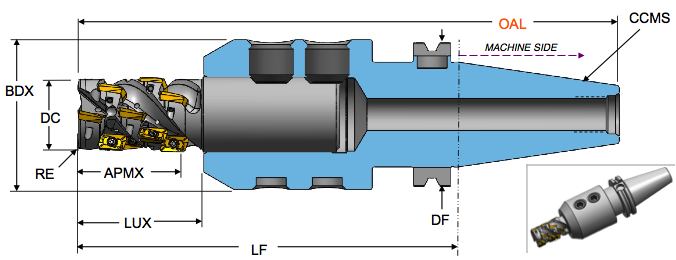
\includegraphics[width=1.0\textwidth]{figures/Cutting Tool Measurement 1.png}
  \caption{Cutting Tool Measurement 1 Diagram}
  \label{fig:Cutting Tool Measurement 1 Diagram}
\end{figure}

\FloatBarrier


\begin{figure}[ht]
  \centering
    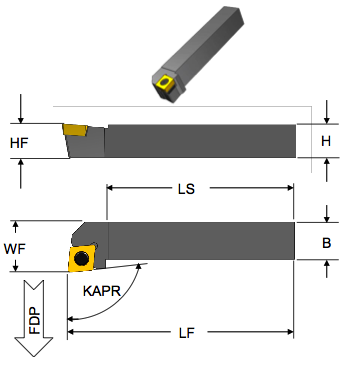
\includegraphics[width=1.0\textwidth]{figures/Cutting Tool Measurement 2.png}
  \caption{Cutting Tool Measurement 2 Diagram}
  \label{fig:Cutting Tool Measurement 2 Diagram}
\end{figure}

\FloatBarrier




\subsubsection{BodyDiameterMax}
\label{sec:BodyDiameterMax}



The largest diameter of the body of a Tool Item.


\texttt{code}: \texttt{BDX}.


\texttt{units}: \texttt{MILLIMETER}.



\subsubsection{BodyLengthMax}
\label{sec:BodyLengthMax}



The distance measured along the X axis from that point of the item closest to the workpiece, including the Cutting Item for a Tool Item but excluding a protruding locking mechanism for an Adaptive Item, to either the front of the flange on a flanged body or the beginning of the connection interface feature on the machine side for cylindrical or prismatic shanks.


\texttt{code}: \texttt{LBX}.


\texttt{units}: \texttt{MILLIMETER}.



\subsubsection{CuttingDiameterMax}
\label{sec:CuttingDiameterMax}



The maximum diameter of a circle on which the defined point Pk of each of the master inserts is located on a Tool Item. The normal of the machined peripheral surface points towards the axis of the Cutting Tool.


\texttt{code}: \texttt{DC}.


\texttt{units}: \texttt{MILLIMETER}.



\subsubsection{DepthOfCutMax}
\label{sec:DepthOfCutMax}



The maximum engagement of the cutting edge or edges with the workpiece measured perpendicular to the feed motion.


\texttt{code}: \texttt{APMX}.


\texttt{units}: \texttt{MILLIMETER}.



\subsubsection{FlangeDiameterMax}
\label{sec:FlangeDiameterMax}



The dimension between two parallel tangents on the outside edge of a flange.


\texttt{code}: \texttt{DF}.


\texttt{units}: \texttt{MILLIMETER}.



\subsubsection{FunctionalLength}
\label{sec:FunctionalLength}



The distance from the gauge plane or from the end of the shank to the furthest point on the tool, if a gauge plane does not exist, to the cutting reference point determined by the main function of the tool. The \block{CuttingTool} functional length will be the length of the entire tool, not a single Cutting Item. Each \block{CuttingItem} can have an independent \block{FunctionalLength} represented in its measurements. 


\texttt{code}: \texttt{LF}.


\texttt{units}: \texttt{MILLIMETER}.



\subsubsection{OverallToolLength}
\label{sec:OverallToolLength}



The largest length dimension of the Cutting Tool including the master insert where applicable.


\texttt{code}: \texttt{OAL}.


\texttt{units}: \texttt{MILLIMETER}.



\subsubsection{ProtrudingLength}
\label{sec:ProtrudingLength}



The dimension from the yz-plane to the furthest point of the Tool Item or Adaptive Item measured in the -X direction.


\texttt{code}: \texttt{LPR}.


\texttt{units}: \texttt{MILLIMETER}.



\subsubsection{ShankDiameter}
\label{sec:ShankDiameter}



The dimension of the diameter of a cylindrical portion of a Tool Item or an Adaptive Item that can participate in a connection.


\texttt{code}: \texttt{DMM}.


\texttt{units}: \texttt{MILLIMETER}.



\subsubsection{ShankHeight}
\label{sec:ShankHeight}



The dimension of the height of the shank.


\texttt{code}: \texttt{H}.


\texttt{units}: \texttt{MILLIMETER}.



\subsubsection{ShankLength}
\label{sec:ShankLength}



The dimension of the length of the shank.


\texttt{code}: \texttt{LS}.


\texttt{units}: \texttt{MILLIMETER}.



\subsubsection{UsableLengthMax}
\label{sec:UsableLengthMax}



Maximum length of a Cutting Tool that can be used in a particular cutting operation including the non-cutting portions of the tool.


\texttt{code}: \texttt{LUX}.


\texttt{units}: \texttt{MILLIMETER}.



\subsubsection{Weight}
\label{sec:Weight}



The total weight of the Cutting Tool in grams. The force exerted by the mass of the Cutting Tool.


\texttt{code}: \texttt{WT}.


\texttt{units}: \texttt{GRAM}.


